\documentclass[10pt,letter]{article}
\usepackage{amsmath}
\usepackage{amssymb}
\usepackage{graphicx}
\usepackage{setspace}
\onehalfspacing
\usepackage{fullpage}
\newcommand{\R}{\mathbb{R}}	
\newcommand{\inner}{\langle\cdot,\cdot\rangle}
\newcommand{\inr}[2]{\langle #1, #2\rangle}
\newcommand\norm[1]{\left\lVert#1\right\rVert}

\begin{document}


\title{ACM104 Problem Set \#5 Solutions}

\author{Timur Kuzhagaliyev}

%\date{16th November, 2017}
 
\maketitle 

\section*{Problem 1}
See attached \texttt{ps5problem1Kuzhagaliyev.m} and relevant plot for solutions.


\section*{Problem 2}
Let $h_{n-1}(x)$ be $n$th monic Hermite polynomial, then:
\begin{align*}
h_0(x) \quad &=\; 1
\\\\
h_1(x) \quad &=\; x - \frac{\inr{x}{1}}{\norm{1}^2}
\\ \quad &=\; x
\\\\
h_2(x) \quad &=\; x^2 - \frac{\inr{x^2}{1}}{\norm{1}^2} - \frac{\inr{x^2}{x}}{\norm{x}^2} \cdot x
\\ \quad &=\; x^2 - \frac{\sqrt{2 \pi}}{\sqrt{2 \pi}} - 0
\\ \quad &=\; x^2 - 1
\\\\
h_3(x) \quad &=\; x^3 - \frac{\inr{x^3}{1}}{\norm{1}^2} - \frac{\inr{x^3}{x}}{\norm{x}^2} \cdot x - \frac{\inr{x^3}{x^2 - 1}}{\norm{x^2 - 1}^2} \cdot (x^2 - 1)
\\ \quad &=\; x^3 - 0 - \frac{3 \sqrt{2 \pi}}{\sqrt{2 \pi}} \cdot x - 0
\\ \quad &=\; x^3 - 3 x
\\\\
h_4(x) \quad &=\; x^4 - \frac{\inr{x^4}{1}}{\norm{1}^2} - \frac{\inr{x^4}{x}}{\norm{x}^2} \cdot x - \frac{\inr{x^4}{x^2 - 1}}{\norm{x^2 - 1}^2} \cdot (x^2 - 1) - \frac{\inr{x^4}{x^3 - 3x}}{\norm{x^3 - 3 x}^2} \cdot (x^3 - 3x)
\\ \quad &=\; x^4 - \frac{3\sqrt{2\pi}}{\sqrt{2\pi}} - 0 - \frac{12 \sqrt{2\pi}}{2\sqrt{2\pi}} \cdot (x^2 - 1) - 0
\\ \quad &=\; x^4 - 3 - 6(x^2 - 1)
\\ \quad &=\; x^4 - 6x^2 + 3
\end{align*}

\pagebreak

\section*{Problem 3}

The case with $\inr{x}{y}_1$ is easy - we just need to find the cross product of $v_1$ and $v_2$. The resultant vector will be orthogonal to both of them, and hence orthogonal to any linear combination of the two. Then, the span of the resultant vector will be our $W^\bot_1$.

\begin{align*}
u_1 = v_1 \times v_2 = 
\left[ {\begin{array}{c}
 2 \cdot 1 - 0 \\
 3 \cdot 2 - 1 \\
 0 - 2 \cdot 2 \\
\end{array} } \right]
= 
\left[ {\begin{array}{c}
 2 \\
 5 \\
 -4 \\
\end{array} } \right]
\quad \Rightarrow \quad W^\bot_1 = span (u_1) = span(
\left[ {\begin{array}{c}
 2 \\
 5 \\
 -4 \\
\end{array} } \right]
)
\end{align*}

For $\inr{x}{y}_2$ we can define two equations using the weighted inner product and the two vectors:
\begin{align*}
\inr{u}{v_1} = 0 &\quad \Rightarrow \quad 1 \cdot x + 2 \cdot 2 \cdot y + 3 \cdot 3 \cdot z = x + 4y + 9z = 0 
\\
\inr{u}{v_2} = 0 &\quad \Rightarrow \quad 2 \cdot x + 0 + 3 \cdot 1 \cdot z = 2x + 3z = 0
\end{align*}
We can solve this system of equations to find the general equation for $u \in W^\bot_2$:
\begin{align*}
x = -\frac{3}{2}z \quad \Rightarrow \quad &-\frac{3}{2}z + 4y +9z = 0
\\ & y = -\frac{15}{8}z
\\\\
z = 1 \quad \Rightarrow \quad x = -\frac{3}{2},\;\; y = -\frac{15}{8} \quad \Rightarrow \quad u_2 =
\left[ {\begin{array}{c}
 -\frac{3}{2} \\
 -\frac{15}{8} \\
 1 \\
\end{array} } \right]
\quad \Rightarrow \quad W^\bot_2 = span (u_2) = span(
\left[ {\begin{array}{c}
 -\frac{3}{2} \\
 -\frac{15}{8} \\
 1 \\
\end{array} } \right]
)
\end{align*}

\pagebreak

\section*{Problem 4}

\begin{align*}
A &=
\left[ {\begin{array}{ccc}
 0 & 0 & -1 \\
 0 &  1 & 0 \\
 1 &  0 & 0 \\
\end{array} } \right]
\end{align*}

The eigenvalues of this matrix are the solutions to the equation $\textrm{det} (A - \lambda I) = 0$:
\begin{gather*}
\textrm{det}
\left[ {\begin{array}{ccc}
 -\lambda & 0 & -1 \\
 0 &  1-\lambda & 0 \\
 1 &  0 & -\lambda \\
\end{array} } \right]
= 0
\\ \Downarrow
\end{gather*}
\begin{align*}
-\lambda(-\lambda)(1-\lambda) - 1 (-1 + \lambda)\quad  &= \quad 0
\\
-\lambda^3 + \lambda^2 - \lambda + 1 \quad &= \quad 0
\end{align*}
By inspection we can conclude that $\lambda = 1$ is a root and hence $(\lambda - 1)$ is a factor, what lets us factorise the equation:
\begin{align*}
(\lambda - 1)(-\lambda^2 -1) \quad &= \quad 0
\\
\lambda = 1 \quad \textrm{OR} \quad -\lambda^2 -1 &= 0
\\
\lambda^2 &= -1
\\
\lambda &= \pm\, i
\end{align*}
$-1$, $i$ and $-i$ are the three distinct eigenvalues of A. We've seen in our equation that all of them had algebraic multiplicity of one. We can find the corresponding eigenvectors:
\begin{gather*}
Av = \lambda v \quad \Rightarrow \quad 
\begin{aligned}
-z = \lambda x
\\
y = \lambda y
\\
x = \lambda z
\end{aligned}
\end{gather*}
\begin{gather*}
\lambda = 1 \quad \Rightarrow \quad
\begin{aligned}
-z = x
\\
y = y
\\
x = z
\end{aligned}
\quad \Rightarrow \quad
\begin{aligned}
x = 0
\\
y = \alpha
\\
z = 0
\end{aligned}
\end{gather*}
\begin{gather*}
\lambda = i \quad \Rightarrow \quad
\begin{aligned}
-z = xi
\\
y = yi
\\
x = zi
\end{aligned}
\quad \Rightarrow \quad
\begin{aligned}
x = zi
\\
y = 0
\end{aligned}
\end{gather*}
\begin{gather*}
\lambda = -i \quad \Rightarrow \quad
\begin{aligned}
-z = -xi
\\
y = -yi
\\
x = -zi
\end{aligned}
\quad \Rightarrow \quad
\begin{aligned}
x = -zi
\\
y = 0
\end{aligned}
\end{gather*}

From the general equations of the vectors corresponding to the eigenvalues, we can conclude that each eigenvalue has a geometric multiplicity of one, hence all eigenvalues are complete. This implies that $A$ is complete. We can also see that generated eigenvectors span entire $\mathbb{C}^3$.

\section*{Problem 5}

\begin{align*}
A &=
\left[ {\begin{array}{ccc}
 0 & 1 & 0 \\
 0 &  1 & 1 \\
 0 &  -1 & 1 \\
\end{array} } \right]
\end{align*}

\paragraph{a)} By a simple calculation we can figure out that the radii of all Gerschgorin disks in this case are 1. The centres for the two possible disks are $(0, 0)$ and $(1, 0)$:
\\\\
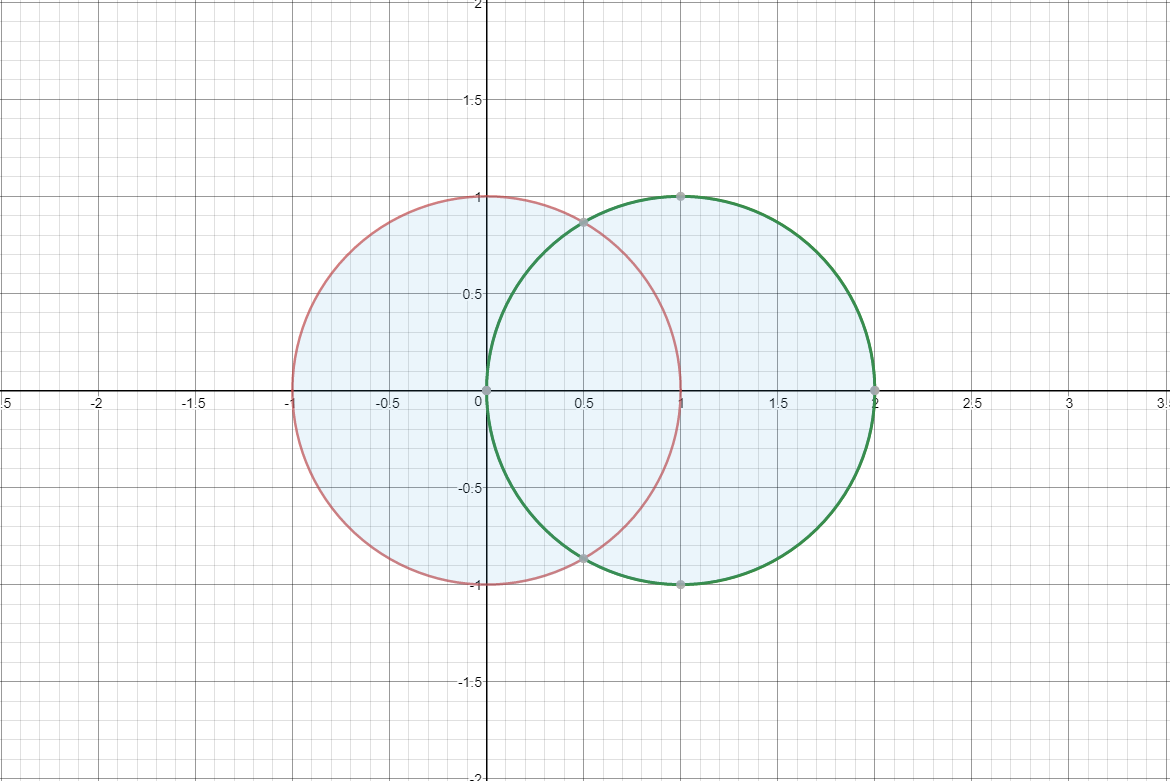
\includegraphics[width=\textwidth,height=\textheight,keepaspectratio]{ps5problem5a.png}

\pagebreak

\paragraph{b)} By Gerschgorin theorem, we know that $spec(A) \subset D_A$ and $spec(A^T) \subset D_{A^T}$. We also know that eigenvalues of $A$ are the solutions for the equation $det(A - \lambda I) = 0$ and that the eigenvalues of $A^T$ satisfy $det(A^T - \lambda I) = 0$. But $det(A^T - \lambda I) = det((A - \lambda I)^T) = det(A - \lambda I)$ since determinant of a matrix is equal to the determinant of its transpose, so $A$ and $A^T$ have the same eigenvalues. This means $spec(A) = spec(A^T)$, hence both  $spec(A) \subset D_A$ and $spec(A) \subset D_{A^T}$ should hold. From this we can conclude that  $spec(A) \subset D_A \cap D_{A^T}$.


\paragraph{c)} Using the refined Gerschgorin domain, we only have one unit circle centred at $(1, 0)$:
\\\\
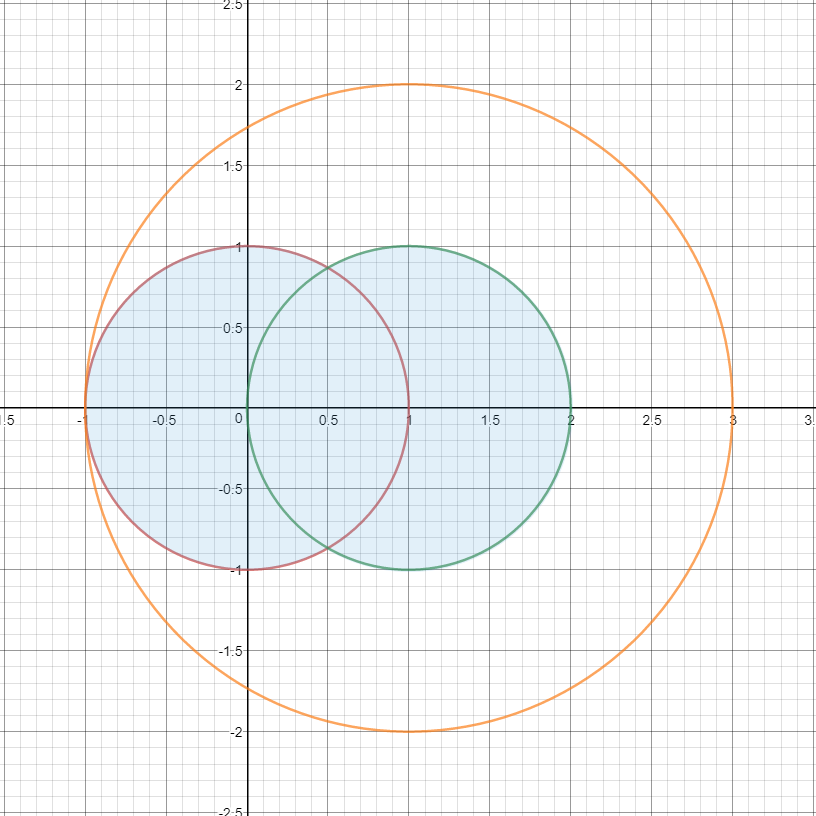
\includegraphics[width=\textwidth,height=\textheight,keepaspectratio]{ps5problem5c.png}

\pagebreak

\paragraph{d)}

The eigenvalues of this matrix are the solutions to the equation $\textrm{det} (A - \lambda I) = 0$:
\begin{gather*}
\textrm{det}
\left[ {\begin{array}{ccc}
 -\lambda & 1 & 0 \\
 0 &  1-\lambda & 1 \\
 0 &  -1 & 1-\lambda \\
\end{array} } \right]
= 0
\\ \Downarrow
\end{gather*}
\begin{gather*}
-\lambda ((1 - \lambda)^2 + 1) - 0 + 0 = 0
\\
-\lambda (\lambda^2 - 2\lambda + 1 + 1) = 0
\\
-\lambda (\lambda^2 - 2\lambda + 2) = 0
\\
-\lambda (\lambda - 1 + i) (\lambda - 1 - i) = 0
\\
\lambda = 0 \quad \textrm{OR} \quad \lambda = 1 - i \quad \textrm{OR} \quad \lambda = 1 + i
\end{gather*}

The eigenvalues of A are $0$, $1-i$ and $1+i$, which indeed lie within the refined Gerschgorin domain.

\end{document}